\documentclass[12pt]{article}
\usepackage[a4paper, total={6in, 8in}]{geometry}
\usepackage{amsfonts}
\usepackage{amsmath,amssymb,trimclip,adjustbox}
\usepackage{breqn}
\usepackage{pgfplots}
\usepackage{hyperref}
\usepackage{tabularray}
\usepackage{polski}
\usepackage[utf8]{inputenc}

\setlength{\parindent}{0pt}
\setlength{\textheight}{650pt}
\setlength{\oddsidemargin}{0pt}
\setlength{\textwidth}{480pt}


\author{Michał Puchyr}
\title{Sprawozdanie z ćw 84 \\
WYZNACZANIE DŁUGOŚCI FALI ŚWIETLNEJ
ZA POMOCĄ SIATKI DYFRAKCYJNEJ}

\begin{document}
\maketitle

\section{Cel ćwiczenia}
\begin{itemize}
    \item Wyznaczenie długości fali emisji lasera lub innego źródła światła
    monochromatycznego
    \item Wyznaczenie stałej siatki dyfrakcyjnej
\end{itemize}

\section{Opis ćwiczenia}
\subsection{Wstęp teoretyczny}

Działanie siatki dyfrakcyjnej polega na wykorzystaniu zjawiska dyfrakcji i interferencji światła do uzyskania jego widma. 
W tym celu pomiędzy źródłem światła a ekranem umieszcza się siatkę dyfrakcyjną. 
Na ekranie uzyskuje się w ten sposób widmo światła.

Przyrządy i materiały wykorzystane do pomiarów : 

\begin{itemize}
    \item Transmisyjne siatki dyfrakcyjne (S) : typ „A” -50 linii na milimetr oraz typ „B”
    \item Laser emitujący zielone światło (PM)
    \item Ekran ze skalą milimetrową (E)
    \item Ława optyczna ze skalą milimetrową
    \item Szczelina (O)
\end{itemize}

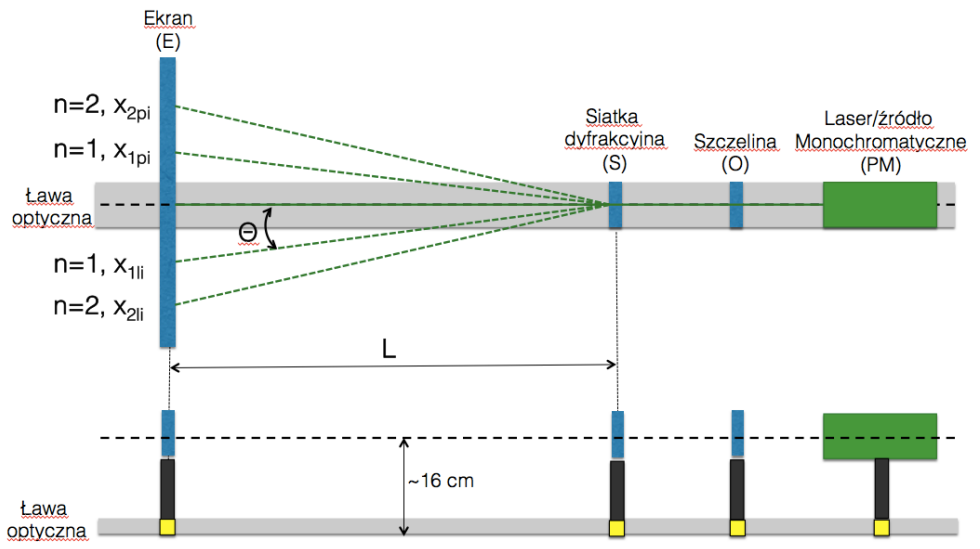
\includegraphics[scale = 0.63]{schemat.png} \\
Schemat układu eksperymentalnego

\section{Pomiary układu}

\begin{table}[!ht]
    \centering
    \begin{tabular}{|l|l|l|l|l|l|l|}
    \hline
    \multicolumn{7}{|l|}{Wyniki pomiarów dla wyznaczenia dł. fali linii monochromatycznej źródła} \\
    \hline
        L$_i$(mm) & u(L$_i$)(mm) & n & x$_{lni}$(mm) & u(x$_{lni}$)(mm) & x$_{lpi}$(mm) & u(x$_{lpi}$)(mm) \\ \hline
        300 & 0,58 & 1 & 8 & 2 & 8 & 2 \\
        ~ & 0,58 & 2 & 17 & 2 & 17 & 2 \\ 
        ~ & 0,58 & 3 & 24 & 2 & 24 & 2 \\ \hline
        350 & 0,58 & 1 & 9 & 2 & 9 & 2 \\
        ~ & 0,58 & 2 & 19 & 2 & 19 & 2 \\ 
        ~ & 0,58 & 3 & 28 & 2 & 28 & 2 \\ \hline
        400 & 0,58 & 1 & 11 & 2 & 11 & 2 \\ 
        ~ & 0,58 & 2 & 22 & 2 & 22 & 2 \\ 
        ~ & 0,58 & 3 & 33 & 2 & 32 & 2 \\ \hline
        450 & 0,58 & 1 & 13 & 2 & 13 & 2 \\ 
        ~ & 0,58 & 2 & 24 & 2 & 24 & 2 \\ 
        ~ & 0,58 & 3 & 37 & 2 & 37 & 2 \\ \hline
        500 & 0,58 & 1 & 14 & 2 & 14 & 2 \\ 
        ~ & 0,58 & 2 & 27 & 2 & 26 & 2 \\ 
        ~ & 0,58 & 3 & 40 & 2 & 40 & 2 \\ \hline
    \end{tabular}
\end{table}

\begin{table}[!ht]
    \centering
    \begin{tabular}{|l|l|l|l|l|l|}
    \hline
    \multicolumn{6}{|l|}{Wyniki pomiarów dla wyznaczenia stałej siatki dyfrakcyjnej} \\
    \hline
        L$_i$(mm) & u(L$_i$)(mm) & x$_{li}$(mm) & u(x$_{li}$)(mm) & x$_{pi}$(mm) & u(x$_{pi}$)(mm) \\ \hline
        50 & 0,58 & 32 & 2 & 32 & 2 \\ \hline
        80 & 0,58 & 49 & 2 & 49 & 2 \\ \hline
        110 & 0,58 & 69 & 2 & 69 & 2 \\ \hline
        140 & 0,58 & 87 & 2 & 87 & 2 \\ \hline
        170 & 0,58 & 105 & 2 & 106 & 2 \\ \hline
        200 & 0,58 & 125 & 2 & 125 & 2 \\ \hline
        230 & 0,58 & 143 & 2 & 144 & 2 \\ \hline
        260 & 0,58 & 162 & 2 & 162 & 2 \\ \hline
        290 & 0,58 & 181 & 2 & 181 & 2 \\ \hline
        320 & 0,58 & 200 & 2 & 200 & 2 \\ \hline
        350 & 0,58 & 218 & 2 & 217 & 2 \\ \hline
        380 & 0,58 & 237 & 2 & 238 & 2 \\ \hline
        410 & 0,58 & 255 & 2 & 255 & 2 \\ \hline
        440 & 0,58 & 275 & 2 & 275 & 2 \\ \hline
        470 & 0,58 & 295 & 2 & 295 & 2 \\ \hline
    \end{tabular}
\end{table}

\section{Wyniki obliczeń}

\begin{table}[!ht]
    \centering
    \begin{tabular}{|l|l|l|l|l|l|l|}
    \hline
    \multicolumn{7}{|l|}{Wyniki obliczeń dla wyznaczenia dł. fali linii monochromatycznej źródła} \\
    \hline
        L$_{n,i}$(mm) & u(L$_{n,i}$)(mm) & $\overline{x}_{n,i}$ & u($\overline{x}_{ini}$)(mm) & $\sin \Theta$ & u($\sin \Theta$) & $\lambda(nm)$ \\ \hline
        300 & 0,58 & 8 & 2 & 0,027 & 0,007 & 540,00 \\ \hline
        300 & 0,58 & 17 & 2 & 0,057 & 0,007 & 570,00 \\ \hline
        300 & 0,58 & 24 & 2 & 0,080 & 0,007 & 533,34 \\ \hline
        350 & 0,58 & 9 & 2 & 0,026 & 0,006 & 520,00 \\ \hline
        350 & 0,58 & 19 & 2 & 0,055 & 0,006 & 550,00 \\ \hline
        350 & 0,58 & 28 & 2 & 0,080 & 0,006 & 533,34 \\ \hline
        400 & 0,58 & 11 & 2 & 0,028 & 0,005 & 560,00 \\ \hline
        400 & 0,58 & 22 & 2 & 0,055 & 0,005 & 550,00 \\ \hline
        400 & 0,58 & 33 & 2 & 0,081 & 0,005 & 540,00 \\ \hline
        450 & 0,58 & 13 & 2 & 0,029 & 0,005 & 580,00 \\ \hline
        450 & 0,58 & 24 & 2 & 0,054 & 0,005 & 540,00 \\ \hline
        450 & 0,58 & 37 & 2 & 0,082 & 0,005 & 546,67 \\ \hline
        500 & 0,58 & 14 & 2 & 0,028 & 0,004 & 560,00 \\ \hline
        500 & 0,58 & 27 & 2 & 0,053 & 0,004 & 530,00 \\ \hline
        500 & 0,58 & 40 & 2 & 0,080 & 0,004 & 533,34 \\ \hline
        \multicolumn{6}{|l|}{Wartość średnia: $\overline{\lambda}(nm)=$} & 545,78 \\ \hline
        \multicolumn{6}{|l|}{Odchylenie standardowe: $u(\overline{\lambda})(nm)=$} & 58,58 \\ \hline
    \end{tabular}
\end{table}

\begin{table}[!ht]
    \centering
    \begin{tabular}{|l|l|l|l|l|}
    \hline
    \multicolumn{5}{|l|}{Wyniki obliczeń dla wyznaczenia stałej siatki dyfrakcyjnej} \\
    \hline
        L$_i$(mm) & $\overline{x}_i$(mm) & u($\overline{x}_i$)(mm) & $\sin \Theta$ & u$_c(\sin \Theta)$ \\ \hline
        50 & 32 & 2 & 0,540 & 0,025 \\ \hline
        80 & 49 & 2 & 0,523 & 0,016 \\ \hline
        110 & 69 & 2 & 0,532 & 0,012 \\ \hline
        140 & 87 & 2 & 0,528 & 0,009 \\ \hline
        170 & 106 & 2 & 0,530 & 0,008 \\ \hline
        200 & 125 & 2 & 0,530 & 0,007 \\ \hline
        230 & 144 & 2 & 0,531 & 0,006 \\ \hline
        260 & 162 & 2 & 0,529 & 0,005 \\ \hline
        290 & 181 & 2 & 0,530 & 0,005 \\ \hline
        320 & 200 & 2 & 0,530 & 0,004 \\ \hline
        350 & 218 & 2 & 0,529 & 0,004 \\ \hline
        380 & 238 & 2 & 0,531 & 0,004 \\ \hline
        410 & 255 & 2 & 0,529 & 0,004 \\ \hline
        440 & 275 & 2 & 0,530 & 0,003 \\ \hline
        470 & 295 & 2 & 0,532 & 0,003 \\ \hline
    \multicolumn{4}{|l|}{Wartość średnia : $\overline{\sin \Theta}=$} & 0,530 \\ \hline
    \multicolumn{4}{|l|}{Odchylenie standardowe : u($\overline{\sin \Theta})=$} & 0,008 \\ \hline
    \multicolumn{4}{|l|}{$d(\mu m)$} & 1029,26 \\ \hline
    \multicolumn{4}{|l|}{$u_c(d)(\mu m)=$} & 111,47 \\ \hline
    \end{tabular}
\end{table}

\subsection{Przykładowe obliczenia}

Obliczenie średniej wartości odległości linii dyfrakcyjnej od pozycji
zerowego rzędu dyfrakcji : 

$$ \overline{x}_{n,i} = \frac{x_{nli} + x_{npi}}{2} = \frac{17 + 17}{2} = 17[mm]$$

$$ u(\overline{x}_{n,i}) = \frac{u(x_{nli}) + u(x_{npi})}{2} = \frac{2 + 2}{2} = 2[mm] $$

Obliczenie sinusa kąta ugięcia :

$$ \sin \Theta_{n,i} = \frac{\overline{x}_{n,i}}{\sqrt{\overline{x}^{2}_{n,i} + L^{2}_i}}
= \frac{8}{\sqrt{8^2 + 300^2}} = 0.02665 \approx 0,027 $$

$$ u_c(\sin \Theta_{n,i}) = \sqrt{\left(\frac{L_i \overline{x}_{n,i}}{\left(L^2_i + \overline{x}_{n,i}\right)^{\frac{3}{2}}}\right)^2 u^2(L) + 
\left(\frac{L^2_i}{(L^2_i + \overline{x}^2_{n,i})^{\frac{3}{2}}}\right)^2 u^2(\overline{x}_{n,i})} = $$

$$ = \sqrt{\left( \right)} $$

\end{document}